\documentclass[state=Report]{mcidoc}

\usepackage{mcidoc-local}
\newtoks\StudentName
\newtoks\StudentID
\newtoks\Supervisor
\newtoks\Cohort
\newtoks\Group
\newtoks\Lecturer

\StudentName={TODO: Vorname Nachname}
\StudentID={TODO: Matrikelnummer}
\Supervisor={TODO: Betreuer}
\Cohort={Abschlussprojekt 2026}
\Group={nil}
\Lecturer={Programmieren I}

\SetMCI{%
StudentName = {Prefix = {}, Name = {TODO: Vorname Nachname}, Postfix = {}},
StudentID = {TODO: Matrikelnummer},
Degree = {MSc},
Language = DE,
Department = {MECH},
Title = {Simulation des Energiebedarfs eines E-Bikes anhand von GPS-Streckendaten},
Report = {%
Lecture = {Programmieren I},
Cohort = {Abschlussprojekt 2026},
Group = {unset},
Mode = {Assignment},
},%
Report/ToC = {Primary = set, Figures = set, Tables = set},
}


\RequirePackage[backend=bibtex,style=ieee]{biblatex}
\addbibresource{references.bib}

\graphicspath{{figures/generated/}{figures/architecture/}}

\begin{Abstract}{DE}
Das Abschlussprojekt implementiert eine datengetriebene E-Bike-Simulation auf Basis realer GPS-Streckendaten. Aus einer semikolonseparierten CSV-Datei werden Zeit, Position, Hoehe und Temperatur eingelesen und in Strecke, Geschwindigkeit, Beschleunigung, Steigung und Kurs umgerechnet. Darauf aufbauend berechnet das Programm die fuer die Fahrt benoetigte Antriebskraft, Leistung, das Raddrehmoment und den Motorstrom. Eine zeitbasierte Glättung der Geschwindigkeit kann optional aktiviert werden, um GPS-Rauschen und starke Beschleunigungsspitzen zu reduzieren. Die Simulation fuehrt ein LiPo- und ein NMC-Akkupack mit derselben Fahrstrecke durch und speichert den Verlauf von Leistung, Drehmoment, Strom, Spannung und Ladezustand. Fuer den vorliegenden Datensatz ergibt sich eine Strecke von 94.27\,km, eine Fahrzeit von 4.55\,h und ein End-SoC von 0\,\% fuer beide Akkutypen, weil der Akku im Verlauf der Fahrt leer wird.
\end{Abstract}

\begin{document}

\chapter{Einleitung}
\label{ch:einleitung}

Das Abschlussprojekt untersucht die Frage, wie viel Energie ein E-Bike auf einer real gefahrenen Route benoetigt. Ausgangspunkt ist keine synthetische Lastkurve, sondern eine GPS-Aufzeichnung mit Zeitstempeln, Position, Hoehe und Temperatur. Dadurch entsteht ein datengetriebenes Modell, das die reale Topografie und das Fahrverhalten der Strecke direkt in die Simulation uebernimmt.

Die Motivation fuer einen solchen Ansatz liegt in der Kopplung mehrerer physikalischer Einfluesse. Die benoetigte Antriebskraft haengt nicht nur von der Geschwindigkeit ab, sondern auch von der Beschleunigung, der Steigung, der Fahrmasse und dem Luftwiderstand. Gerade bei einer Route mit wechselnder Hoehe und vielen kurzen Messabstaenden kann GPS-Rauschen zu stark schwankenden Geschwindigkeiten fuehren. Das Projekt versucht deshalb, die Messdaten aufzubereiten, die Fahrwiderstaende zu bestimmen und darauf aufbauend zwei unterschiedliche Akkutechnologien zu vergleichen.

Das Projektziel ist klar abgegrenzt: Es wird kein vollstaendiges Fahrdynamikmodell mit Fahrerleistung, Wind, Antriebsregelung oder Motorwirkungsgrad simuliert. Stattdessen berechnet die Software aus den GPS-Daten die fuer die Strecke notwendige mechanische Leistung und speist diesen Lastverlauf in ein LiPo- und ein NMC-Akkupack ein. Die zentrale Forschungsfrage lautet damit nicht, wie das Fahrzeug vorwaerts simuliert wird, sondern wie sich eine gegebene Fahrt energetisch auf unterschiedliche Speichertechnologien auswirkt.

\section{Beitrag des Projekts}

Das Programm verbindet Datenverarbeitung, Physik und Visualisierung in einer einzigen Pipeline. Die GPS-Rohdaten werden eingelesen, in Kinematikgroessen umgerechnet, optional geglaettet und anschliessend durch ein E-Bike-Modell und zwei Akku-Varianten verarbeitet. Die Ergebnisse werden sowohl numerisch als auch grafisch ausgegeben: als HTML-Karten, als PNG-Diagramme und als Logdatei. Die technische Dokumentation orientiert sich an der verwendeten Klasse \cite{mcidoc_template}, waehrend das hier beschriebene Programm selbst im Repository des Abschlussprojekts liegt \cite{abschlussprojekt_repo}.

\section{Dokumentation im Bericht}

Die folgenden Kapitel beschreiben zunachst die Anforderungen und die Repository-Struktur, dann die objektorientierte Architektur, die GPS- und Kinematikberechnung, die Geschwindigkeitsglaettung, das physikalische Modell, die Akku- und Motormodelle, den Simulationsablauf sowie die erzeugten Ausgaben. Abschliessend werden die Tests, die realen Simulationsergebnisse und die Grenzen des Modells diskutiert.

\chapter{Anforderungen}
\label{ch:anforderungen}

Das aktuelle Projekt implementiert die im Quellcode nachweisbaren Kernfunktionen einer routenbasierten E-Bike-Simulation. Die Anforderungen lassen sich in bereits umgesetzte Kernfunktionen, sichtbare Erweiterungen und naheliegende Folgearbeiten trennen.

\section{Implementierte Kernfunktionen}

\begin{itemize}
  \item Einlesen einer GPS-CSV-Datei mit den Spalten \texttt{time}, \texttt{lat}, \texttt{lon}, \texttt{ele} und \texttt{temperature}.
  \item Berechnung von Zeitdifferenzen, Distanz, Geschwindigkeit, Steigung, Kurswinkel, Kompassrichtung und Beschleunigung.
  \item Optionale Geschwindigkeitsglaettung mit konfigurierbarer Zeitbasis.
  \item Berechnung der Antriebskraft, mechanischen Leistung, des Raddrehmoments und des Motorstroms.
  \item Simulation des Ladezustands, der Klemmenspannung und der temperaturabhaengigen Akkuparameter fuer LiPo und NMC.
  \item Erzeugung von HTML-Karten, PNG-Diagrammen und einer Logdatei.
\end{itemize}

\section{Erweiterungen gegenueber einer Minimalversion}

Das Projekt geht ueber eine reine Streckenauswertung hinaus. Die GPS-Daten werden nicht nur gelesen, sondern in eine zeitlich konsistente Kinematik ueberfuehrt. Ausserdem verwendet das Programm eine abstrakte Akkobasis, damit der Simulator mit mehreren Akkutypen arbeiten kann. Die Luftdichte wird nicht konstant angesetzt, sondern aus Hoehe und Temperatur abgeschaetzt, und ein Bremswiderstandsmodell faengt Ueberschuesse beim Laden ab.

\section{Nicht implementierte oder bewusst ausgesparte Funktionen}

Mehrere inhaltlich naheliegende Erweiterungen sind im aktuellen Code nicht enthalten und werden daher im Bericht auch nicht behauptet: direkte Fahrerleistung, Windmodell, Motorwirkungsgrad, Rueckspeisung in ein reales Ladenetz, Sensordaten von Leistung oder Drehmoment sowie eine aktive Regelung des Antriebs. Ebenso gibt es keine Pauschalbegrenzung der Geschwindigkeit oder Beschleunigung; die Verarbeitung arbeitet ausschliesslich daten- und segmentbasiert.

\section{Technische Randbedingungen}

Die Software ist fuer einen lokalen Python-Workflow mit virtueller Umgebung ausgelegt. Installiert werden die in \texttt{requirements.txt} genannten Pakete sowie LuaLaTeX. Die Ausgabedateien werden im Verzeichnis \texttt{output/} erzeugt; der Bericht selbst verwendet davon getrennte Kopien der wichtigsten Plot-Dateien im Verzeichnis \texttt{report/figures/generated/}.

\chapter{Projektstruktur}
\label{ch:projektstruktur}

Das Repository ist flach organisiert: Jedes Modul hat eine klar benannte Aufgabe. Das erleichtert Simulation und Wartung, weil GPS-Verarbeitung, Fahrzeugphysik, Motorlogik, Akkuverhalten und Visualisierung getrennt bleiben.

\section{Übersicht der Komponenten}

\begin{table}[htbp]
\centering
\caption{Wesentliche Komponenten des Repositories und ihre Verantwortung}
\label{tab:komponenten}
\begin{tabularx}{\textwidth}{@{}lX@{}}
\toprule
Komponente & Verantwortung \\
\midrule
\texttt{main.py} & Programmstart, Logging, Laden der Konfiguration, Erzeugen von Track, Fahrzeug, Motor und Akkus sowie Start der Simulation. \\
\texttt{gps\_track.py} & Einlesen der GPS-CSV, Berechnung von Distanz, Geschwindigkeit, Steigung, Kurs, Kompassrichtung und Beschleunigung sowie Kartenerzeugung. \\
\texttt{speed\_smoothing.py} & Laden der Glättungskonfiguration, Segmentierung und zeitbasierte Glättung der Geschwindigkeitskurve. \\
\texttt{ebike.py} & Fahrzeugphysik mit Luft-, Hang-, Roll- und Beschleunigungsanteilen. \\
\texttt{motor.py} & Umrechnung von Drehmoment in Motorstrom über die Motorkonstante. \\
\texttt{ebike\_simulator.py} & Schrittweise Simulation der Fahrt und Aufzeichnung der Ergebnisprofile. \\
\texttt{battery\_base.py} & Abstrakte Schnittstelle für Batteriemodelle. \\
\texttt{battery\_pack.py} & Gemeinsame Akku-Funktionalität, SoC-Integration, Temperaturkorrektur und Begrenzung. \\
\texttt{lipo\_battery.py} & LiPo-spezifische OCV-Kennlinie und Packparametrisierung. \\
\texttt{nmc\_battery.py} & NMC-spezifische OCV-Kennlinie und Packparametrisierung. \\
\texttt{akkutemperatur.py} & Temperaturabhängige Korrektur von Innenwiderstand und Kapazität. \\
\texttt{luftdichte.py} & Schätzung der Luftdichte aus Höhe und Temperatur. \\
\texttt{bremswiderstand.py} & Umrechnung von überschüssigem Strom in dissipierte Leistung. \\
\texttt{plot\_utils.py} & Matplotlib-Plots für Höhenprofil, Zeitverläufe und SoC-Vergleich. \\
\texttt{wetterdaten.py} & Abfrage von Temperatur, Wind und Niederschlag für Streckenpunkte über die Open-Meteo-API. \\
\texttt{app.py} / \texttt{webapp/} & Flask-Web-Anwendung: Simulation und Parameterstudien im Browser bedienbar. \\
\texttt{data/} & Eingabedaten und Konfigurationsdateien. \\
\texttt{tests/} & Unittest-Suite für Glättung, Kinematik und Simulator-Kompatibilität. \\
\texttt{output/} & Laufzeit-Ausgaben des Programms. \\
\bottomrule
\end{tabularx}
\end{table}

\section{Zentrale Klassen und Funktionen}

{\small
\begin{xltabular}{\textwidth}{@{}lp{4.4cm}X@{}}
\caption{Ausgewählte Klassen und ihre öffentlichen Methoden mit Kurzkommentar}
\label{tab:klassen-methoden}\\
\toprule
Klasse & Methode / Attribut & Kommentar \\
\midrule
\endfirsthead
\caption[]{Ausgewählte Klassen und ihre öffentlichen Methoden mit Kurzkommentar (Fortsetzung)}\\
\toprule
Klasse & Methode / Attribut & Kommentar \\
\midrule
\endhead
\midrule
\multicolumn{3}{r}{\textit{Fortsetzung auf der nächsten Seite}} \\
\endfoot
\bottomrule
\endlastfoot
\texttt{GPSTrack} & \texttt{GPSTrack(pfad, smoothing\_config=None)} & Konstruktor; liest die CSV ein und berechnet daraus sofort die gesamte Kinematik (Distanz, Geschwindigkeit, Steigung, Kurs, Beschleunigung). \\
 & \texttt{gesamtstrecke\_km()} & Summiert alle Distanzsegmente \texttt{distanz\_m} zur Gesamtstrecke. \\
 & \texttt{durchschnittsgeschwindigkeit\_kmh()} & Gesamtstrecke geteilt durch Gesamtzeit. \\
 & \texttt{gesamtzeit\_s()} & Zeitspanne zwischen erstem und letztem GPS-Punkt. \\
 & \texttt{hoehenmeter\_anstieg()} & Summe aller positiven Höhendifferenzen \(\Delta h_i\). \\
 & \texttt{hoehenmeter\_abstieg()} & Summe aller negativen Höhendifferenzen (als Betrag). \\
 & \texttt{haufigste\_kompassrichtung()} & Häufigster Wert der Spalte \texttt{kompassrichtung}. \\
 & \texttt{kennzahlen\_ausgeben()} & Schreibt die wichtigsten Streckenkennzahlen in Konsole und Logdatei. \\
 & \texttt{smoothing\_kennzahlen()} & Vergleicht Roh- und geglättete Geschwindigkeit/Beschleunigung (z.\,B. maximale Differenz). \\
 & \texttt{karte\_erstellen(...)} & Erstellt eine nach Geschwindigkeit eingefärbte interaktive HTML-Karte (Folium). \\
 & \texttt{orte\_ermitteln(anzahl\_wegpunkte=8)} & Reverse Geocoding ausgewählter Streckenpunkte zu Adressen über Nominatim/geopy. \\
 & \texttt{karte\_erstellen\_geopandas(...)} & Statische, farbcodierte GIS-Karte (GeoPandas/Matplotlib) als Alternative zur Folium-Karte. \\
 & \texttt{karte\_erstellen\_geopandas\_einfach(...)} & Vereinfachte GeoPandas-Karte ohne Einfärbung, gesamte Strecke als ein Liniensegment. \\
\midrule
\texttt{SpeedSmoothingConfig} & \texttt{from\_yaml(path)} & Lädt die YAML-Konfiguration und prüft die Werte auf Plausibilität. \\
 & Attribut \texttt{max\_reasonable\_speed\_ms} & Aus \texttt{max\_reasonable\_speed\_kmh} umgerechnete Plausibilitätsgrenze in m/s. \\
\midrule
\texttt{EBike} & \texttt{from\_yaml(pfad)} & Erzeugt ein \texttt{EBike}-Objekt aus \texttt{data/bike\_config.yaml} inkl. Default-Werten. \\
 & \texttt{luftwiderstand\_N(v, rho)} & Luftwiderstandskraft \(F_{\mathrm{Luft}} = \tfrac{1}{2}\rho\, c_{\mathrm{w}}A\, v^2\). \\
 & \texttt{hangabtriebskraft\_N(phi)} & Hangabtriebskraft \(F_{\mathrm{Hang}} = m g \sin(\varphi)\) aus der Steigung. \\
 & \texttt{beschleunigungskraft\_N(a)} & Trägheitskraft \(F_{\mathrm{Beschl.}} = m a\). \\
 & \texttt{rollwiderstand\_N(phi)} & Rollwiderstand \(F_{\mathrm{Roll}} = c_{\mathrm{R}} m g \cos(\varphi)\). \\
 & \texttt{antriebskraft\_N(v, a, phi, rho)} & Summe der vier Einzelkräfte; zentrale Kraftbilanz des Fahrzeugmodells. \\
 & \texttt{leistung\_W(F, v)} & Mechanische Leistung \(P = F v\). \\
 & \texttt{drehmoment\_Nm(F)} & Raddrehmoment \(M = F r\) mit dem Radradius \(r\). \\
 & \texttt{punkt\_auswerten(v, a, phi, rho)} & Bündelt Kraft, Leistung und Drehmoment für einen GPS-Punkt in einem Aufruf; wird vom Simulator pro Zeitschritt genutzt. \\
\midrule
\texttt{Motor} & \texttt{Motor(motorkonstante\_Nm\_A=1.5)} & Konstruktor; speichert die Motorkonstante \(k_{\mathrm{m}}\) in Nm/A. \\
 & \texttt{get\_current\_draw(torque\_Nm)} & Rechnet Drehmoment in Motorstrom um: \(I = M / k_{\mathrm{m}}\). \\
\midrule
\texttt{BatteryBase} & \texttt{apply\_current(...)}, \texttt{voltage(...)} & Abstrakte Methoden (ABC); legen nur fest, dass jede Akku-Klasse SoC-Update und Spannungsabfrage bereitstellen muss. \\
\midrule
\texttt{BatteryPack} & \texttt{set\_temperatur(temperature\_c)} & Setzt die aktuelle Akkutemperatur, die anschliessend \(R_{\mathrm{int}}\) und \(C_{\mathrm{nom}}\) korrigiert. \\
 & \texttt{apply\_current(current, duration)} & Konkrete SoC-Integration inkl. Ladungs-/Entladungsbegrenzung, Bremswiderstandslogik und Fehlermeldung bei leerem Akku. \\
 & \texttt{voltage(current)} & Klemmenspannung \(U = U_{\mathrm{OC}}(\mathrm{SoC}) - R_{\mathrm{int}} I\), temperaturkorrigiert. \\
 & \texttt{is\_empty()} / \texttt{is\_full()} & Prüft, ob SoC an der unteren bzw. oberen Grenze (0 bzw. 1) liegt. \\
\midrule
\texttt{LiPoBatteryPack} & \texttt{LiPoBatteryPack(capacity\_nom\_Ah, initial\_soc=1.0, n\_parallel=1)} & Konstruktor; skaliert Kapazität und Innenwiderstand mit \texttt{n\_parallel}. \\
 & \texttt{\_ocv(soc)} & Überschreibt die Leerlaufspannung durch lineare Interpolation der LiPo-Messkennlinie (\texttt{numpy.interp}). \\
\texttt{NMCBatteryPack} & \texttt{NMCBatteryPack(capacity\_nom\_Ah, initial\_soc=1.0, n\_parallel=1)} & Konstruktor; analog zu \texttt{LiPoBatteryPack}. \\
 & \texttt{\_ocv(soc)} & Analog für die NMC-spezifische Messkennlinie. \\
\midrule
\texttt{EBikeSimulator} & \texttt{EBikeSimulator(track, bike, motor, battery)} & Konstruktor; speichert die vier Objekte per Assoziation, ohne sie zu verändern. \\
 & \texttt{simulate()} & Läuft den GPS-Track Punkt für Punkt ab, berechnet Kraft/Leistung/Strom und wendet ihn auf den Akku an; liefert das Ergebnis-DataFrame. \\
 & \texttt{maximalleistung\_W()} & Maximum des aufgezeichneten Leistungsprofils. \\
 & \texttt{bremswiderstand\_energie\_Wh()} & Über die gesamte Fahrt integrierte, am Bremswiderstand dissipierte Energie. \\
 & \texttt{endladezustand\_prozent()} & Letzter Wert des SoC-Profils in Prozent. \\
 & \texttt{zusammenfassung\_ausgeben()} & Gibt Akkuzustand, Maximalleistung, End-SoC und dissipierte Energie auf der Konsole aus. \\
\end{xltabular}
}

\section{Dateien und Ausgaben}

Die Eingabedaten liegen unter \texttt{data/}. Ergebnisse entstehen zur Laufzeit unter \texttt{output/}, Unterordner für Plots werden dabei automatisch angelegt. Für den Bericht wurden die PNGs zusätzlich nach \texttt{report/figures/generated/} kopiert, damit der PDF-Build unabhängig vom letzten Programmlauf funktioniert.

\chapter{Softwarearchitektur und OOP}
\label{ch:softwarearchitektur}

Die Architektur des Projekts folgt einer klaren Trennung zwischen Datenquelle, physikalischem Modell, Energieversorgung und Visualisierung. Die Klassen kooperieren ueber Assoziationen und Vererbung, aber die fachliche Verantwortung bleibt in getrennten Modulen gebuendelt.

\section{Objektorientierte Struktur}

\texttt{BatteryBase} definiert die abstrakte Schnittstelle fuer alle Akku-Modelle. \texttt{BatteryPack} liefert die gemeinsame Implementierung mit SoC-Integration und Temperaturkorrektur. \texttt{LiPoBatteryPack} und \texttt{NMCBatteryPack} spezialisieren nur die Leerlaufspannungskennlinie sowie die physikalischen Packparameter. Dadurch kann \texttt{EBikeSimulator} den Akku polymorph verwenden, ohne den konkreten Typ kennen zu muessen.

\texttt{GPSTrack} ist die Datenquelle fuer die Simulation. \texttt{EBike} modelliert die Fahrphysik, \texttt{Motor} die Umrechnung von Drehmoment in Strom. Der Simulator verbindet diese Objekte und fuehrt die Strecke zeitdiskret aus. So entstehen klare Zustaendigkeiten: Datenaufbereitung in \texttt{GPSTrack}, Physik in \texttt{EBike}, elektrische Umrechnung im \texttt{Motor}, Energiespeicherung im Akku und Ablaufsteuerung im Simulator.

\section{Klassendiagramm}

\begin{figure}[htbp]
\centering
\begin{tikzpicture}[node distance=14mm and 18mm, every node/.style={font=\small}, box/.style={draw, rounded corners, align=center, minimum width=28mm, minimum height=9mm}, arr/.style={-Latex, thick}]
  \node[box] (batterybase) {BatteryBase};
  \node[box, below=of batterybase] (batteryPack) {BatteryPack};
  \node[box, below left=of batteryPack] (lipo) {LiPoBatteryPack};
  \node[box, below right=of batteryPack] (nmc) {NMCBatteryPack};

  \node[box, right=40mm of batterybase] (sim) {EBikeSimulator};
  \node[box, above right=of sim] (track) {GPSTrack};
  \node[box, right=of sim] (bike) {EBike};
  \node[box, below right=of sim] (motor) {Motor};
  \node[box, below=of sim] (battery) {BatteryBase};

  \draw[arr] (batterybase) -- (batteryPack);
  \draw[arr] (batteryPack) -- (lipo);
  \draw[arr] (batteryPack) -- (nmc);

  \draw[arr] (sim) -- (track);
  \draw[arr] (sim) -- (bike);
  \draw[arr] (sim) -- (motor);
  \draw[arr] (sim) -- (battery);
\end{tikzpicture}
\caption{UML-ahnliche Sicht auf die wesentlichen Klassen und Beziehungen}
\label{fig:klassendiagramm}
\end{figure}

Das Diagramm zeigt die im Code sichtbare Struktur: Vererbung nach unten bei den Batterien und Assoziationen vom Simulator zu den vier zentralen Objekten. Die Richtung der Pfeile ist absichtlich einfach gehalten, weil der Schwerpunkt auf der inhaltlichen Architektur liegt, nicht auf einer vollstaendigen UML-Notation.

\section{Daten- und Kontrolltrennung}

Die Datenverarbeitung ist von der Simulation entkoppelt. Das Programm liest die CSV und bereitet sie in \texttt{GPSTrack} auf, erzeugt danach ein Objekt des E-Bikes und des Motors und fuehrt dann die Simulation fuer jeden Akkutyp separat aus. Diagramme und Karten sind rein nachgelagerte Ausgaben; sie beeinflussen das Simulationsmodell nicht.

\chapter{GPS- und Kinematikberechnung}
\label{ch:gps-kinematik}

Die GPS-Eingabe ist eine semikolonseparierte CSV mit den Spalten \texttt{time}, \texttt{lat}, \texttt{lon}, \texttt{ele} und \texttt{temperature}. Die Zeitstempel liest \texttt{pandas.to\_datetime} als UTC ein \cite{pandas_docs}. Die Zeilen müssen bereits zeitlich sortiert sein, die Berechnung nutzt dann nur aufeinanderfolgende Punkte.

\section{Zeit und Distanz}

Für zwei aufeinanderfolgende Punkte $i-1$ und $i$ gilt im Code:
\begin{equation}
\Delta t_i = t_i - t_{i-1}
\end{equation}
\begin{equation}
\Delta s_i = 2 R \arcsin\left(\sqrt{a}\right)
\end{equation}
mit
\begin{equation}
 a = \sin^2\!\left(\frac{\Delta \varphi}{2}\right) + \cos(\varphi_{i-1})\cos(\varphi_i)\sin^2\!\left(\frac{\Delta \lambda}{2}\right)
\end{equation}
und $R = \SI{6371000}{\metre}$ als mittlerem Erdradius. Diese Haversine-Formel ist für die Distanzberechnung vorgegeben und wird direkt in \texttt{GPSTrack\_distanz\_haversine()} umgesetzt.

Aus Distanz und Zeit folgt die Rohgeschwindigkeit:
\begin{equation}
 v_i = \frac{\Delta s_i}{\Delta t_i}
\end{equation}

Ist \(\Delta t_i \le 0\), setzt das Projekt die Rohgeschwindigkeit auf \SI{0}{\metre\per\second} und markiert das Intervall als ungültig. So vermeidet die Berechnung eine Division durch null, ohne Datenpunkte zu verlieren.

\section{Steigung, Kurs und Kompassrichtung}

Die Höhendifferenz wird als
\begin{equation}
\Delta h_i = h_i - h_{i-1}
\end{equation}
verwendet. Daraus entsteht die Steigung in Grad als
\begin{equation}
\varphi_i = \arctan\!\left(\frac{\Delta h_i}{\Delta s_i}\right)
\end{equation}
falls $\Delta s_i > 0$ ist, sonst $0$. 
Der Kurswinkel (englisch \emph{initial bearing}) folgt aus Breiten- und Längengrad
zweier aufeinanderfolgender Punkte über die Formel
\begin{equation}
    \theta_i = \operatorname{atan2}\Big(
        \sin(\Delta\lambda)\cos(\varphi_i),\;
        \cos(\varphi_{i-1})\sin(\varphi_i) - \sin(\varphi_{i-1})\cos(\varphi_i)\cos(\Delta\lambda)
    \Big)
    \label{eq:kurswinkel}
\end{equation}
mit $\Delta\lambda = \lambda_i - \lambda_{i-1}$. Da $\operatorname{atan2}$ Werte im Bereich
$(-180\si{\degree}, 180\si{\degree}]$ liefert, wird das Ergebnis anschlie{\ss}end über
$\theta_i \bmod 360\si{\degree}$ auf $[0\si{\degree}, 360\si{\degree})$ normalisiert.

Aus dem normalisierten Kurswinkel ergibt sich die Kompassrichtung durch Rundung auf
den nächstgelegenen $45\si{\degree}$-Sektor:
\begin{equation}
    \text{Sektorindex} = \operatorname{round}\!\left(\frac{\theta_i}{45\si{\degree}}\right) \bmod 8
    \label{eq:kompasssektor}
\end{equation}
Die acht Sektoren $0$ bis $7$ entsprechen dabei den Richtungen N, NO, O, SO, S, SW, W
und NW, beginnend bei $0\si{\degree}$ (Norden) und im Uhrzeigersinn fortlaufend. Ein
Kurswinkel von z.\,B. $80\si{\degree}$ ergibt so Sektor $2$, also O.

\section{Beschleunigung}

Die Beschleunigung entsteht nicht aus einer einfachen Differenz zweier aufeinanderfolgender Geschwindigkeitswerte, sondern segmentweise aus der aktiven Geschwindigkeitskurve. Der Grund: Bei ungleichmäßigen Zeitabständen -- wie sie bei GPS-Aufzeichnungen üblich sind -- würde eine reine Vorwärtsdifferenz das Ergebnis unnötig empfindlich gegenüber genau dem Punkt machen, an dem sie ausgewertet wird. \texttt{beschleunigung\_aus\_geschwindigkeit()} verwendet deshalb eine zentrale Differenz: Für einen Punkt $i$ wird die Geschwindigkeitsänderung zwischen dem Vorgänger- und dem Nachfolgerpunkt durch die Zeit zwischen den beiden Intervallmitten geteilt. Das mittelt den Einfluss beider Nachbarn und reagiert dadurch weniger empfindlich auf einen einzelnen verrauschten Messwert als eine reine Vorwärts- oder Rückwärtsdifferenz.

An den Segmentgrenzen gibt es keinen Vorgänger bzw. Nachfolger im selben Segment; dort setzt die Funktion die Beschleunigung am ersten Punkt auf null und verwendet am letzten Punkt eine einseitige (rückwärtige) Differenz. Segmente werden dabei nicht überschritten: Eine Beschleunigung wird nie über eine grosse Zeitlücke hinweg berechnet, weil das einen physikalisch bedeutungslosen Wert ergeben würde (z.\,B. eine sehr kleine Beschleunigung über eine mehrminütige Aufzeichnungspause).

\section{Wichtige DataFrame-Spalten}

Diese Spalten bilden die Grundlage für die weiteren Kapitel:
\texttt{dt\_s}, \texttt{distanz\_m}, \texttt{steigung\_grad}, \texttt{kurs\_grad}, \texttt{kompassrichtung}, \texttt{geschwindigkeit\_roh\_ms}, \texttt{geschwindigkeit\_geglaettet\_ms}, \texttt{geschwindigkeit\_ms}, \texttt{beschleunigung\_roh\_ms2}, \texttt{beschleunigung\_geglaettet\_ms2}, \texttt{beschleunigung\_ms2} sowie die Filterspalten der Glättung. Der Simulator nutzt später nur \texttt{geschwindigkeit\_ms} und \texttt{beschleunigung\_ms2}.

\chapter{Geschwindigkeitsglättung}
\label{ch:glaettung}

GPS-Positionen schwanken oft leicht, besonders bei kurzen Zeitintervallen. Da die Geschwindigkeit hier aus Distanz durch Zeit berechnet wird, erzeugen kleine Zeitdifferenzen schnell hohe Spitzen -- die wiederum auf Beschleunigung und Leistung durchschlagen. Das Projekt bietet daher eine zeitbasierte Glättung, die sich in \texttt{data/speed\_smoothing\_config.yaml} ein- oder ausschalten lässt.

\section{Konfigurationsparameter}

Die aktuelle Konfiguration enthält diese Werte:
\begin{table}[htbp]
\centering
\caption{Parameter der Geschwindigkeitsglättung (\texttt{data/speed\_smoothing\_config.yaml})}
\label{tab:smoothing-config}
\begin{tabularx}{\textwidth}{@{}llX@{}}
\toprule
Parameter & Aktueller Wert & Bedeutung \\
\midrule
\texttt{enabled} & \texttt{true} & Schaltet die Glättung ein oder aus; bei \texttt{false} bleiben die Rohwerte aktiv. \\
\texttt{min\_interval\_s} & 0.5\,s & Untere Schranke für gültige Filterstützstellen; kürzere Intervalle gelten als zu unsicher für eine Geschwindigkeitsberechnung und werden ausgeschlossen. \\
\texttt{max\_gap\_s} & 30.0\,s & Zeitlücke, ab der ein neues Segment beginnt, damit über Aufzeichnungslücken hinweg nicht geglättet oder interpoliert wird. \\
\texttt{median\_window\_s} & 15.0\,s & Zeitfenster des zeitbasierten Medianfilters; größer bedeutet stärkere Glättung, aber trägere Reaktion auf echte Geschwindigkeitsänderungen. \\
\texttt{time\_constant\_s} & 3.0\,s & Zeitkonstante \(\tau\) der exponentiellen Glättung; steuert, wie schnell die geglättete Kurve der Rohkurve folgt. \\
\texttt{max\_reasonable\_speed\_kmh} & 60.0\,km/h & Plausibilitätsgrenze für Stützstellen; darüber liegende Rohwerte gelten als Ausreißer und werden aus der Filterbasis entfernt. \\
\bottomrule
\end{tabularx}
\end{table}

\section{Ablauf der Glättung}

Der Algorithmus arbeitet segmentweise und führt die folgenden Schritte aus:
\begin{enumerate}
  \item Rohgeschwindigkeit berechnen.
  \item Ungültige Intervalle erkennen, also \(\Delta t \le 0\).
  \item Sehr kurze Intervalle als ungeeignete Stützstellen markieren.
  \item Grosse Zeitlücken in getrennte Segmente aufteilen.
  \item Unplausible Geschwindigkeiten als Ausreisser markieren.
  \item Einen zeitbasierten Medianfilter anwenden.
  \item Fehlende Werte nur innerhalb des Segments interpolieren.
  \item Eine zeitabhängige exponentielle Glättung vorwärts ausführen.
  \item Die Glättung rückwärts wiederholen.
  \item Beide Verläufe mitteln.
  \item Die Beschleunigung aus der aktiven Geschwindigkeitskurve berechnen.
\end{enumerate}

\paragraph{Warum Segmente statt einer durchgehenden Kurve?} Eine grosse Zeitlücke (länger als \texttt{max\_gap\_s}) bedeutet meist eine echte Aufzeichnungspause, z.\,B. ein Stopp ohne GPS-Fix. Würde der Filter darüber hinweg glätten oder interpolieren, würde er eine Bewegung erfinden, die nie stattgefunden hat. Deshalb beginnt an solchen Lücken ein neues Segment, und jedes Segment wird unabhängig gefiltert.

\paragraph{Warum zuerst Median, dann Exponentialfilter?} Die beiden Filter lösen unterschiedliche Probleme. Der zeitbasierte Median entfernt einzelne, kurze Ausreisser robust, weil ein Median durch einen einzelnen extremen Wert kaum verschoben wird -- anders als ein Mittelwert. Erst danach glättet die exponentielle Filterung die verbleibende, kleinräumige Unruhe der Kurve. Würde man nur exponentiell glätten, würden einzelne GPS-Spitzen die Kurve noch mehrere Sekunden lang nachziehen.

\paragraph{Warum vorwärts UND rückwärts filtern?} Eine einfache exponentielle Glättung reagiert erst NACH einer Geschwindigkeitsänderung -- sie hinkt der echten Kurve zeitlich hinterher (Phasenverzögerung). Filtert man dieselbe Formel zusätzlich auf der umgekehrten Zeitachse, "hinkt" dieser zweite Verlauf in die andere Richtung, er reagiert quasi zu früh. Der Mittelwert aus beiden Richtungen hebt diese Verzögerung weitgehend auf, sodass die geglättete Kurve zeitlich zur echten Bewegung passt statt ihr nur verzögert zu folgen.

\paragraph{Was passiert, wenn ein Segment keine gültige Stützstelle hat?} Bleiben in einem kurzen Segment z.\,B. nur Ausreisser oder zu kurze Intervalle übrig, kann nicht sinnvoll gefiltert werden. In diesem Fall verwendet das Programm für dieses Segment die Rohgeschwindigkeit unverändert weiter und loggt eine Warnung, statt mit leeren oder erfundenen Werten weiterzurechnen.

\section{Mathematische Beschreibung}

Die zeitabhängige Glättung verwendet den Faktor
\begin{equation}
\alpha_i = 1 - \exp\left(-\frac{\Delta t_i}{\tau}\right)
\end{equation}
mit der Zeitkonstante \(\tau\). Daraus folgt die Rekursion
\begin{equation}
 v_{\mathrm{glatt},i}
 = v_{\mathrm{glatt},i-1}
 + \alpha_i\left(v_i - v_{\mathrm{glatt},i-1}\right)
\end{equation}
Die Rückwärtsfilterung nutzt dieselbe Formel auf der umgekehrten Zeitachse; anschliessend werden beide Verläufe gemittelt.

Die Konfiguration wird aus YAML geladen \cite{pyyaml_docs} und vor der Nutzung auf Plausibilität geprüft.

\section{Aktive und passive Spalten}

Das Projekt unterscheidet zwischen Roh-, geglätteter und aktiver Größe. \texttt{geschwindigkeit\_roh\_ms} bleibt immer erhalten, \texttt{geschwindigkeit\_geglaettet\_ms} zeigt das Filterergebnis, \texttt{geschwindigkeit\_ms} ist die für die Simulation aktive Kurve. Analog gilt das für \texttt{beschleunigung\_roh\_ms2}, \texttt{beschleunigung\_geglaettet\_ms2} und \texttt{beschleunigung\_ms2}. Es gibt keine pauschale Begrenzung oder Kappung -- nur Filterstützstellen und Segmente werden gezielt behandelt.

\chapter{Physikalisches E-Bike-Modell}
\label{ch:physik}

Das Fahrzeugmodell in \texttt{ebike.py} berechnet fuer jeden GPS-Punkt die benoetigte Kraft aus Fahrwiderstaenden, Beschleunigung und Steigung. Die Rechnung erfolgt in Fahrtrichtung und nutzt die aus dem GPS-Datensatz abgeleitete Geschwindigkeit und Beschleunigung.

\section{Einzelkraefte}

Der Luftwiderstand folgt im Projekt direkt der bekannten quadratischen Form und entspricht der in der Aerodynamik ueblichen Drag-Gleichung \cite{nasa_drag}:
\begin{equation}
F_{\mathrm{Luft}} = \frac{1}{2}\rho c_{\mathrm{w}}A v^2
\end{equation}
Dabei ist \(\rho\) die Luftdichte, \(c_{\mathrm{w}}A\) die aerodynamische Kennzahl und \(v\) die Geschwindigkeit. Fuer die Luftdichte verwendet das Projekt entweder die ueber \texttt{luftdichte.py} berechnete aktuelle Dichte oder eine konstante Standarddichte, falls Hoehe und Temperatur nicht nutzbar sind.

Die Hangabtriebskraft lautet
\begin{equation}
F_{\mathrm{Hang}} = m g \sin(\varphi)
\end{equation}
und die Beschleunigungskraft
\begin{equation}
F_{\mathrm{Beschleunigung}} = m a
\end{equation}
mit der Gesamtmasse \(m\), der Erdbeschleunigung \(g\), der Steigung \(\varphi\) und der Beschleunigung \(a\).

Der Rollwiderstand wird im Code als
\begin{equation}
F_{\mathrm{Roll}} = c_{\mathrm{R}} m g \cos(\varphi)
\end{equation}
modelliert. Die verwendete Masse setzt sich aus Fahrer- und Fahrradmasse zusammen.

\section{Gesamtkraft und Leistung}

Die Funktion \texttt{EBike.antriebskraft\_N()} bildet die Summe
\begin{equation}
F_{\mathrm{Antrieb}} = F_{\mathrm{Luft}} + F_{\mathrm{Hang}} + F_{\mathrm{Beschleunigung}} + F_{\mathrm{Roll}}
\end{equation}
und damit genau die im Quellcode verwendete Kraft. Aus Kraft und Geschwindigkeit folgt die mechanische Leistung
\begin{equation}
P = F v
\end{equation}
und das Raddrehmoment
\begin{equation}
M = F r
\end{equation}
mit dem Radradius \(r\).

\section{Parameter}

Die Parameter werden aus \texttt{data/bike\_config.yaml} geladen. Aktuell verwendet das Projekt eine Fahrer- und Radmasse von zusammen \SI{80}{\kilogram}, eine aerodynamische Kennzahl von \SI{0.5625}{\square\metre}, einen Raddurchmesser von \SI{27}{\centi\metre} und einen Rollwiderstandskoeffizienten von \num{0.005}. Diese Werte bestimmen gemeinsam mit der GPS-Kinematik die Leistungsanforderung entlang der Strecke.

\chapter{Motor- und Akkumodelle}
\label{ch:motor-akku}

\section{Motor}

Die Klasse \texttt{Motor} bildet eine einfache lineare Umrechnung vom Raddrehmoment auf den Strom ab. Verwendet wird die im Projekt explizit geforderte Motorkonstante:
\begin{equation}
I = \frac{M}{k_{\mathrm{m}}}
\end{equation}
Die Motorkonstante ist in \si{\newton\metre\per\ampere} angegeben. Der Motor ist als eigene Klasse modelliert, damit die Beziehung zwischen mechanischer Last und elektrischem Strom explizit und austauschbar bleibt.

\section{Abstrakte Akku-Schnittstelle}

\texttt{BatteryBase} definiert nur das Interface. Jede konkrete Akku-Klasse muss mindestens die Aktualisierung des Ladezustands und die Berechnung der Klemmenspannung bereitstellen. Diese Abstraktion ist entscheidend fuer den Polymorphismus im Simulator: Der Code arbeitet auf dem Basistyp, nicht auf einer konkreten Unterklasse.

\section{Gemeinsame Akku-Funktionalitaet}

\texttt{BatteryPack} implementiert ein Ersatzschaltbild aus Leerlaufspannung und Innenwiderstand. Der Ladezustand wird ueber die Stromintegration aktualisiert:
\begin{equation}
\mathrm{SoC}_{k+1} = \mathrm{SoC}_k - \frac{I\,\Delta t}{C_{\mathrm{nom}}}
\end{equation}
Die Nennkapazitaet wird von \si{\ampere\hour} nach \si{\ampere\second} umgerechnet. Positiver Strom entlaedt den Akku, negativer Strom laedt ihn. Die Klemmenspannung ergibt sich als
\begin{equation}
U = U_{\mathrm{OC}}(\mathrm{SoC}) - R_{\mathrm{int}} I
\end{equation}
und wird temperaturkorrigiert, wenn eine Temperatur gesetzt wurde.

Temperatur beeinflusst zwei Groessen: Der Innenwiderstand steigt bei kaelteren Temperaturen relativ zur Referenz von \SI{25}{\celsius}, waehrend die nutzbare Kapazitaet sinkt. Beide Korrekturen sind nach unten begrenzt, damit bei extremen Temperaturen keine unrealistische Extrapolation entsteht.

\section{LiPo und NMC}

LiPo- und NMC-Akkus erben beide von \texttt{BatteryPack} und unterscheiden sich nur in der Kennlinie und im Innenwiderstand. Das Projekt verwendet tabellarische Leerlaufspannungskennlinien mit linearer Interpolation \cite{numpy_docs}. Dadurch laesst sich das Verhalten beider Akkus unter identischem Lastprofil direkt vergleichen.

\begin{table}[htbp]
\centering
\caption{Gemeinsamkeiten und Unterschiede der beiden Akkupacks}
\label{tab:lipo-nmc}
\begin{tabularx}{\textwidth}{@{}lXX@{}}
\toprule
Aspekt & LiPoBatteryPack & NMCBatteryPack \\
\midrule
Vererbung & Erbt von \texttt{BatteryPack} & Erbt von \texttt{BatteryPack} \\
Serienschaltung & 10 Zellen & 10 Zellen \\
Innenwiderstand & \SI{8}{\milli\ohm} pro Zelle, skaliert mit \texttt{n\_parallel} & \SI{7}{\milli\ohm} pro Zelle, skaliert mit \texttt{n\_parallel} \\
OCV-Kennlinie & LiPo-Stuetzstellen aus Tabelle & NMC-Stuetzstellen aus Tabelle \\
Interpolation & \texttt{numpy.interp} & \texttt{numpy.interp} \\
Verhalten unter Last & Hoehere Leerlaufspannung bei gleichem SoC & Niedrigere Leerlaufspannung bei gleichem SoC \\
\bottomrule
\end{tabularx}
\end{table}

\section{Bremswiderstand und Rekuperation}

Wenn beim Bergabfahren oder Bremsen ein negativer Motorstrom entsteht, steigt der Ladezustand des Akkus. Ueberschreitet dieser Ladevorgang 100\,\%, wird der zulaessige Strom begrenzt. Der ueberschuessige Strom wird dann ueber den Bremswiderstand in Waerme umgesetzt und in \texttt{letzte\_dissipierte\_leistung\_W} gespeichert. Im aktuellen Datensatz tritt dieser Fall nicht auf; die gespeicherte dissipierte Leistung bleibt in beiden Simulationslaeufen bei null.

\chapter{Simulationsablauf}
\label{ch:simulation}

\section{Aktivitätsdiagramm der Simulation}

Abbildung~\ref{fig:aktivitaetsdiagramm} zeigt den vollständigen Ablauf einer Simulation für einen Akkutyp, von den Eingabedaten bis zu den Ausgaben. \texttt{BatteryPack.apply\_current()} prüft dabei zuerst, ob der Akku leer ist und eine Entladung versucht wird (Abbruch), und erst danach, ob die Ladung 100\,\% überschreiten würde (Bremswiderstandslogik) -- genau in dieser Reihenfolge bildet das Diagramm es ab.

\begin{figure}[htbp]
\centering
\resizebox{\textwidth}{!}{%
\begin{tikzpicture}[
  node distance=7mm and 16mm,
  every node/.style={font=\scriptsize},
  act/.style={draw, rounded corners, align=center, minimum width=42mm, minimum height=7mm, fill=black!3},
  dec/.style={draw, diamond, align=center, inner sep=1pt, aspect=2.2, fill=black!3},
  arr/.style={-Latex, thick},
]
  \node[circle, fill=black, minimum size=2.5mm, inner sep=0] (start) {};
  \node[act, below=of start] (a1) {GPS-Daten und Konfiguration laden};
  \node[act, below=of a1] (a2) {Kinematik berechnen: Distanz, $v$, $a$, Steigung};
  \node[dec, below=of a2] (d1) {Glättung\\aktiviert?};
  \node[act, right=28mm of d1] (a3) {Geschwindigkeit glätten,\\Beschleunigung neu berechnen};
  \node[dec, below=9mm of d1] (m1) {};
  \node[act, below=of m1] (a4) {E-Bike, Motor, Akku erzeugen};
  \node[act, below=of a4] (loop) {Nächsten GPS-Punkt wählen};
  \node[act, below=of loop] (a5) {Luftdichte bestimmen; Kraft, Leistung,\\Drehmoment und Motorstrom berechnen};
  \node[dec, below=of a5] (d2) {Akku leer und\\Entladung nötig?};
  \node[act, right=55mm of d2] (a8) {Simulation abbrechen};
  \node[dec, below=9mm of d2] (m2) {};
  \node[act, below=of m2] (a6) {Ladezustand aktualisieren\\(Stromintegration)};
  \node[dec, below=of a6] (d3) {SoC würde\\$>100\%$ steigen?};
  \node[act, right=28mm of d3] (a7) {Strom begrenzen, Überschuss\\über Bremswiderstand dissipieren};
  \node[dec, below=9mm of d3] (m3) {};
  \node[act, below=of m3] (av) {Spannung berechnen};
  \node[dec, below=of av] (d4) {Weitere\\Punkte?};
  \node[act, below=of d4] (a9) {Kennzahlen, Plots, Karten, Log erzeugen};
  \node[circle, draw, below=of a9, minimum size=3.2mm, inner sep=0] (endc) {};
  \node[circle, fill=black, minimum size=1.8mm, inner sep=0] at (endc) {};

  \draw[arr] (start) -- (a1);
  \draw[arr] (a1) -- (a2);
  \draw[arr] (a2) -- (d1);
  \draw[arr] (d1) -- node[left]{nein} (m1);
  \draw[arr] (d1) -- node[above]{ja} (a3);
  \draw[arr] (a3) |- (m1.east);
  \draw[arr] (m1) -- (a4);
  \draw[arr] (a4) -- (loop);
  \draw[arr] (loop) -- (a5);
  \draw[arr] (a5) -- (d2);
  \draw[arr] (d2) -- node[left]{nein} (m2);
  \draw[arr] (d2) -- node[above]{ja} (a8);
  \draw[arr] (m2) -- (a6);
  \draw[arr] (a6) -- (d3);
  \draw[arr] (d3) -- node[left]{nein} (m3);
  \draw[arr] (d3) -- node[above]{ja} (a7);
  \draw[arr] (a7) |- (m3.east);
  \draw[arr] (m3) -- (av);
  \draw[arr] (av) -- (d4);
  \draw[arr] (d4) -- node[above]{ja} ++(-42mm,0) |- (loop.west);
  \draw[arr] (d4) -- node[left]{nein} (a9);
  \draw[arr] (a8) |- ($(a9.east)+(0,3mm)$) -- (a9.east);
  \draw[arr] (a9) -- (endc);
\end{tikzpicture}%
}
\caption{Aktivitätsdiagramm des Simulationsablaufs für einen Akkutyp}
\label{fig:aktivitaetsdiagramm}
\end{figure}

\section{Warum bricht die Simulation bei leerem Akku ab, statt weiterzurechnen?}

\texttt{EBikeSimulator.simulate()} verarbeitet die Strecke Punkt für Punkt und hält dabei den zuletzt gültigen Index fest. Wirft der Akku beim Entladeversuch einen Fehler (siehe Kapitel~\ref{ch:motor-akku}), stoppt die Schleife an genau dieser Stelle: Das zurückgegebene Ergebnis-DataFrame enthält dann nur die Punkte bis zum Abbruch, nicht die gesamte Strecke. Diese Entscheidung spiegelt die Realität wider -- ein leerer Akku kann keine weitere Fahrt antreiben --, und sie ist der Grund, warum in Kapitel~\ref{ch:ergebnisse} beide Akkus vor dem Streckenende auf 0\,\% SoC fallen: Die Simulation bricht dort ab, wo der Akku tatsächlich leer wäre, statt unrealistisch mit negativem Ladezustand weiterzulaufen.

Die Luftdichte wird pro Punkt einzeln bestimmt und nicht einmalig für die ganze Strecke: Höhe und Temperatur ändern sich während der Fahrt, und schlägt die Berechnung für einen einzelnen Punkt fehl (z.\,B. wegen fehlender Werte), fängt der Simulator das ab und verwendet für diesen einen Punkt die Standarddichte, statt die gesamte Simulation abzubrechen.

\section{Datenfluss}

\begin{figure}[htbp]
\centering
\begin{tikzpicture}[node distance=10mm and 12mm, every node/.style={font=\small}, box/.style={draw, rounded corners, align=center, minimum width=28mm, minimum height=8mm}, arr/.style={-Latex, thick}]
  \node[box] (csv) {GPS-CSV};
  \node[box, below left=of csv] (bikecfg) {Bike-\-Konfiguration};
  \node[box, below right=of csv] (smoothcfg) {Glättungs-\-konfiguration};
  \node[box, below=of csv] (track) {GPSTrack};
  \node[box, below=of track] (kin) {Kinematik und optionale Glättung};
  \node[box, below=of kin] (sim) {EBikeSimulator};
  \node[box, below=of sim] (phys) {EBike + Motor + Akku};
  \node[box, below=of phys] (frames) {Simulations-\-DataFrames};
  \node[box, below=of frames] (out) {Kennzahlen, PNGs, HTML-Karten, Logdatei};

  \draw[arr] (csv) -- (track);
  \draw[arr] (bikecfg) |- (phys.west);
  \draw[arr] (smoothcfg) |- (track.east);
  \draw[arr] (track) -- (kin);
  \draw[arr] (kin) -- (sim);
  \draw[arr] (sim) -- (phys);
  \draw[arr] (phys) -- (frames);
  \draw[arr] (frames) -- (out);
\end{tikzpicture}
\caption{Programmfluss von den Eingabedaten bis zu den Ausgaben}
\label{fig:datenfluss}
\end{figure}

\section{Ablauf in \texttt{main.py}}

Der Programmstart legt die Ausgabeverzeichnisse an und startet das Logging. Danach lädt das Programm Glättungskonfiguration und GPS-Track, gibt die Streckenkennzahlen aus und schreibt eine Karte mit der Streckenfarbe nach Geschwindigkeit.

Als Nächstes entstehen E-Bike, Motor und zwei Akkupacks. Der Simulator läuft dann zweimal -- einmal für LiPo, einmal für NMC -- auf derselben Strecke. Nach jedem Lauf speichert das Programm eine SoC-Karte und das Ergebnis-DataFrame. Zum Schluss erstellt \texttt{plot\_utils.py} die Diagramme.

\section{Übergebene Daten}

Zwischen den Komponenten wandern nur DataFrames, einfache Zahlen und Klassenobjekte. \texttt{GPSTrack} liefert die aufbereiteten Spalten, \texttt{EBikeSimulator} ergänzt Leistungs- und Akkuwerte. So bleibt die Schnittstelle einfach und testbar.

\chapter{Visualisierung und Ausgaben}
\label{ch:visualisierung}

Das Projekt erzeugt zwei Ausgabearten: interaktive HTML-Karten mit Folium und statische PNG-Diagramme mit Matplotlib. Beide greifen nur auf bereits berechnete Daten zu.

\section{HTML-Karten: wie der Streckenplot funktioniert}

Die Karten entstehen in \texttt{GPSTrack.karte\_erstellen()} mit \texttt{folium} \cite{folium_docs}, das eine interaktive Leaflet-Karte im Browser erzeugt. Die Strecke wird dabei nicht als eine einzelne Linie gezeichnet, sondern in einzelne Segmente zwischen je zwei aufeinanderfolgenden GPS-Punkten zerlegt. Jedes Segment bekommt über eine lineare Farbskala (\texttt{branca.colormap}, blau-grün-gelb-rot) eine eigene Farbe, je nach Wert einer wählbaren Spalte -- standardmäßig die Geschwindigkeit, bei den SoC-Karten stattdessen der Ladezustand. So zeigt die Streckenfarbe direkt, wo z.\,B. schnell gefahren wurde oder wo der Akku bereits weit entladen war.

Start- und Zielpunkt erhalten eigene Marker (grün/rot). Wurde zuvor \texttt{orte\_ermitteln()} aufgerufen, zeigen deren Popups die per Reverse Geocoding ermittelte Adresse statt nur \enquote{Start}/\enquote{Ziel}, und zusätzliche blaue Marker markieren die abgefragten Zwischenpunkte. Als Kartenhintergrund dient standardmäßig \texttt{cartodbpositron} statt des klassischen OpenStreetMap-Stils: Der offizielle OSM-Kachelserver verlangt einen Referer-Header, den Browser beim direkten Öffnen einer lokalen HTML-Datei nicht mitschicken -- die Kacheln würden sonst mit einem Zugriffsfehler abgelehnt.

Die Strecke liegt so als farbcodierte Linie in \texttt{output/karte\_strecke.html}. Der Simulator erzeugt zusätzlich zwei SoC-Karten, \texttt{output/karte\_soc\_lipo.html} und \texttt{output/karte\_soc\_nmc.html}, indem dieselbe Funktion auf das jeweilige Ergebnis-DataFrame mit der Spalte \texttt{soc} angewendet wird. Alle Karten lassen sich direkt im Browser öffnen.

\section{PNG-Diagramme}

Die Plots liegen unter \texttt{output/plot/}, erzeugt mit \texttt{matplotlib} \cite{matplotlib_docs}. \texttt{plot\_utils.py} baut dafür die x-Achse aus der kumulierten Distanz (\texttt{distanz\_m.cumsum()}) bzw. aus der seit Fahrtbeginn vergangenen Zeit; die y-Werte kommen direkt aus den in Kapitel~\ref{ch:physik} und \ref{ch:motor-akku} berechneten Spalten. Für den Bericht wurden Kopien nach \texttt{report/figures/generated/} übernommen.

\begin{figure}[htbp]
\centering
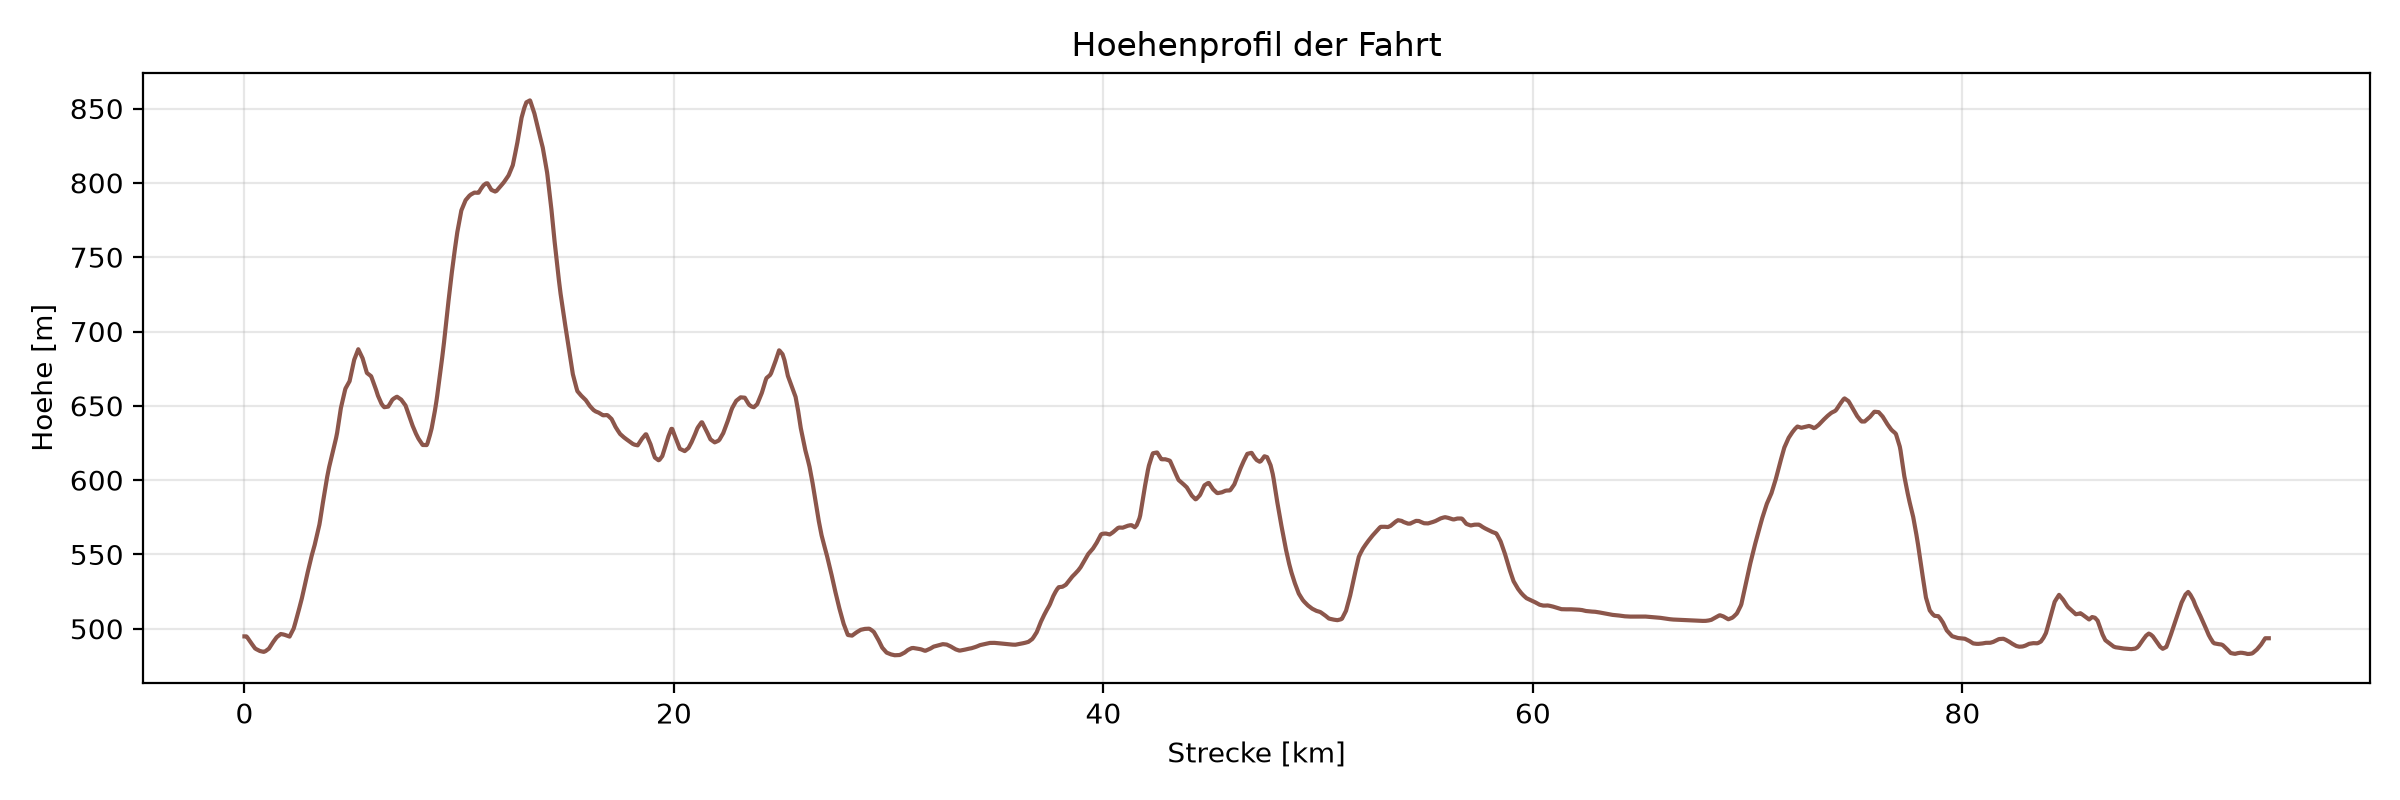
\includegraphics[width=0.9\textwidth]{hoehenprofil_fahrt.png}
\caption{Höhenprofil der betrachteten Route}
\label{fig:hoehenprofil}
\end{figure}

Abbildung~\ref{fig:hoehenprofil} zeigt das Höhenprofil der Strecke. Es ist wichtig für die Leistungs- und Akkuabschätzung, da Steigung und Gefälle direkt in die Hangabtriebskraft eingehen.

\begin{figure}[htbp]
\centering
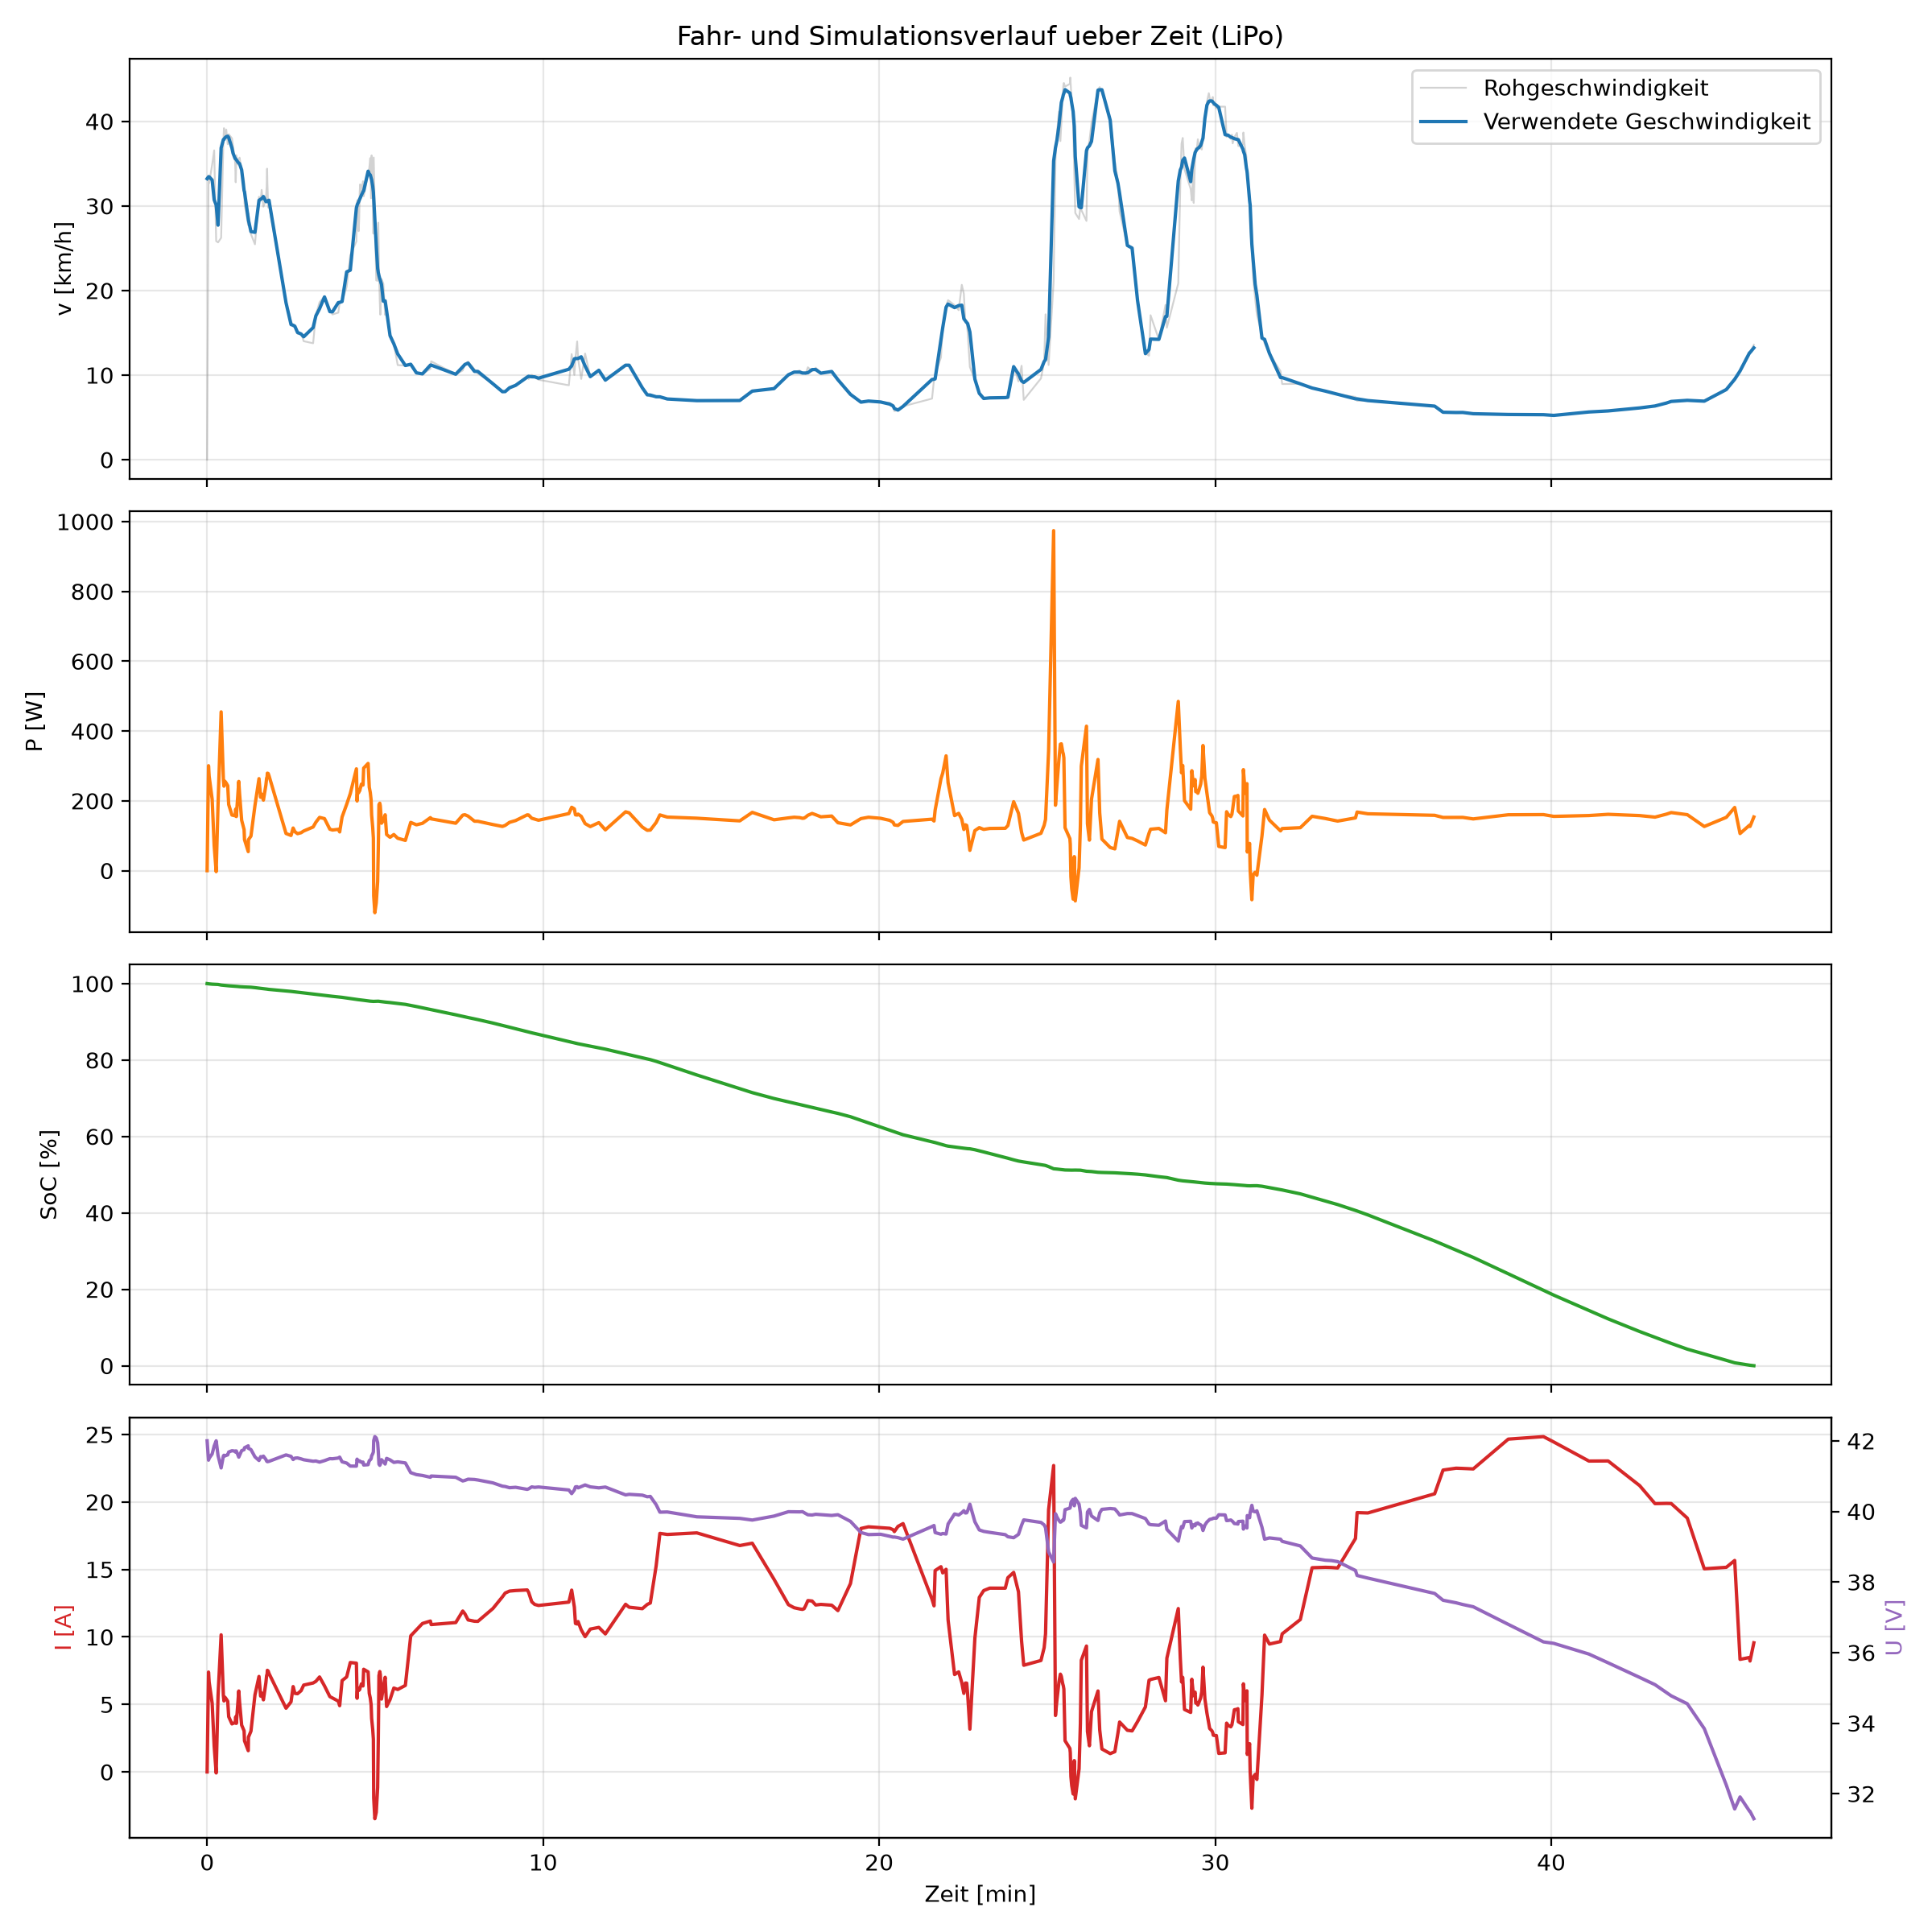
\includegraphics[width=0.9\textwidth]{zeitverlauf_lipo.png}
\caption{Zeitverlauf der Simulationsgrößen für den LiPo-Lauf}
\label{fig:zeitverlauf-lipo}
\end{figure}

Abbildung~\ref{fig:zeitverlauf-lipo} zeigt vier übereinander liegende Diagramme mit gemeinsamer Zeitachse: Geschwindigkeit (mit Rohkurve im Hintergrund, falls Glättung aktiv ist), Leistung, Ladezustand sowie Strom und Spannung auf einer geteilten y-Achse. Leistungsspitzen und Stromverlauf folgen dabei direkt der aktiven Geschwindigkeitskurve. Für NMC entsteht die gleiche Grafik analog.

\begin{figure}[htbp]
\centering
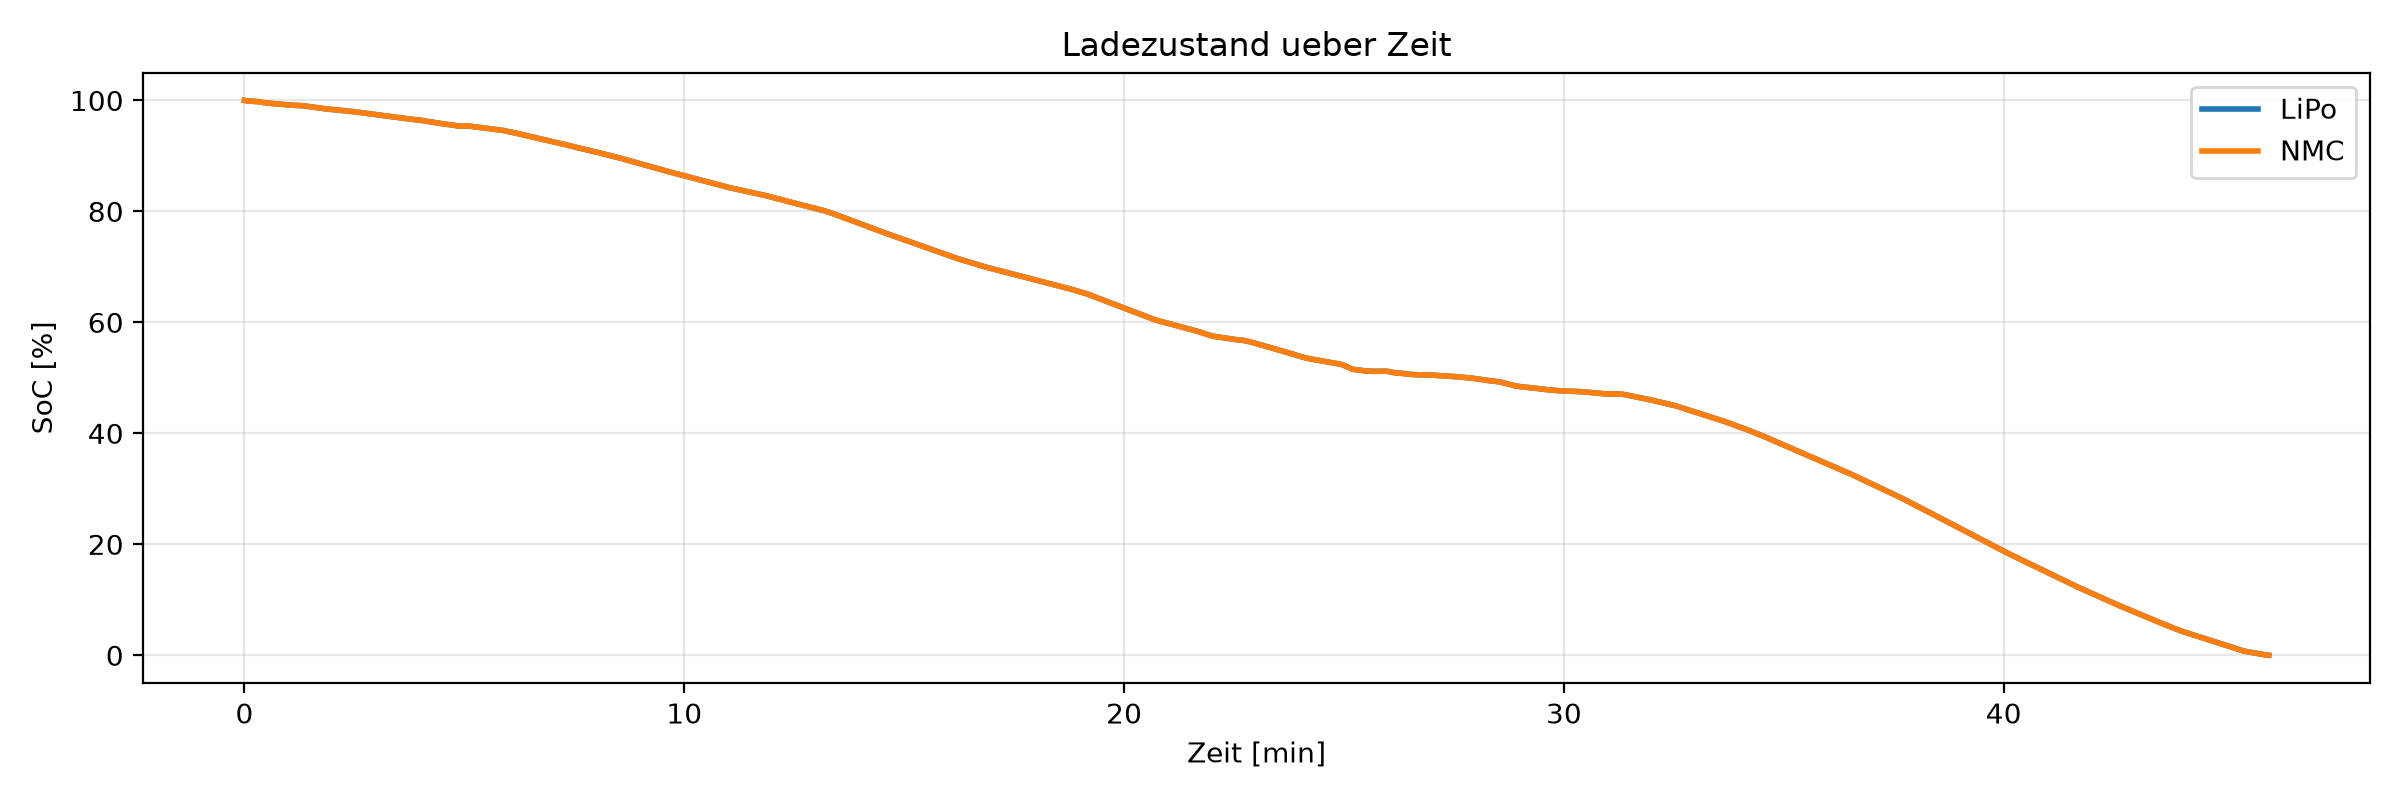
\includegraphics[width=0.9\textwidth]{ladezustand_vergleich.png}
\caption{Vergleich des Ladezustands beider Akkutypen}
\label{fig:soc-vergleich}
\end{figure}

Abbildung~\ref{fig:soc-vergleich} vergleicht beide Akkus im gleichen Fahrprofil. Da der Akku im Datensatz leer wird, laufen beide Kurven bis auf 0\,\% herunter.

\begin{figure}[htbp]
\centering
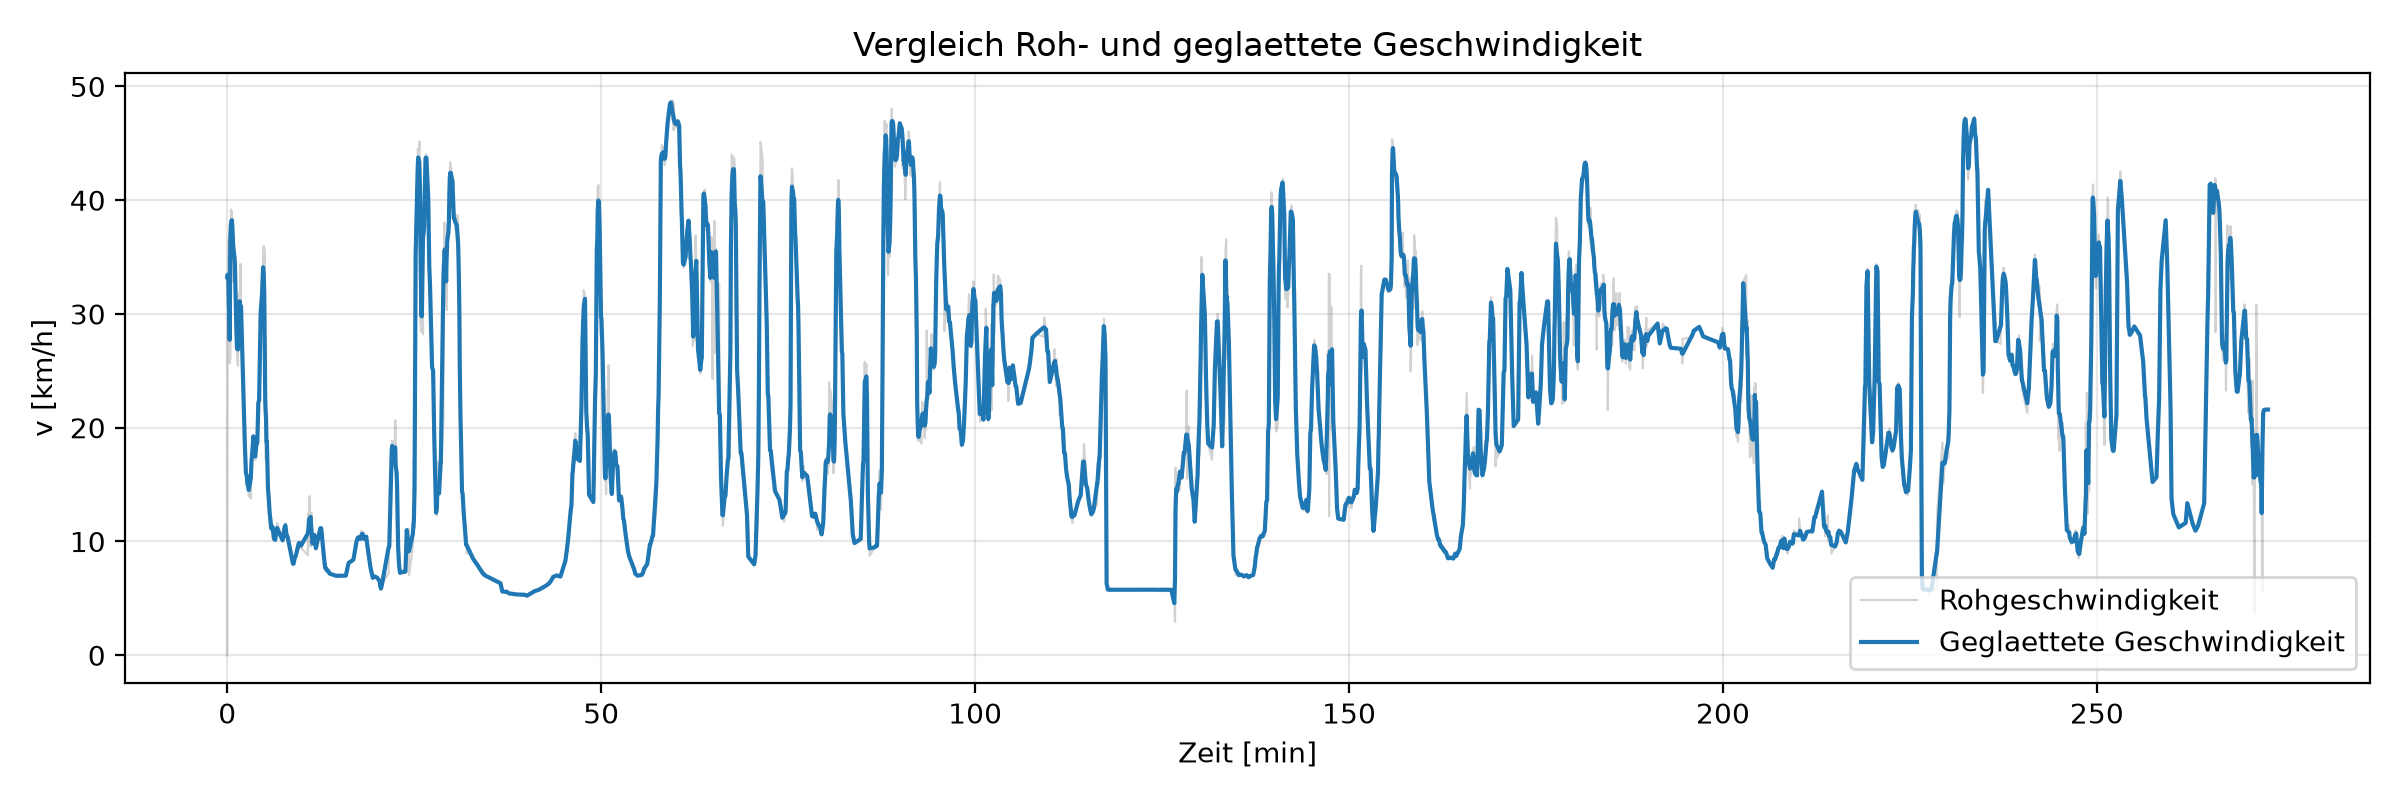
\includegraphics[width=0.9\textwidth]{geschwindigkeit_roh_geglaettet.png}
\caption{Vergleich von Roh- und geglätteter Geschwindigkeit}
\label{fig:speed-comparison}
\end{figure}

Abbildung~\ref{fig:speed-comparison} zeigt den Filtereffekt: Die geglättete Kurve entfernt schnelle Zacken, ohne die Strecke selbst zu verändern.

\section{Logdatei und Verzeichnisse}

Die Logdatei \texttt{output/ebike\_simulation.log} spiegelt die Konsolenausgaben mit Zeitstempeln. Alle Verzeichnisse legt das Programm beim Start automatisch an.

\chapter{Tests und Validierung}
\label{ch:tests}

Das Projekt enthielt im aktuellen Stand zwei Testdateien. Sie pruefen die Konfiguration und das Verhalten der Geschwindigkeitsglättung sowie die Integration mit \texttt{GPSTrack} und dem Simulator.

\section{Ausgefuehrter Testbefehl}

Die Tests wurden mit dem folgenden Befehl ausgefuehrt:

\begin{lstlisting}
python -m unittest discover -s tests -v
\end{lstlisting}

\section{Ergebnis}

Die Test-Suite umfasst 14 Einzeltests. Alle 14 Tests sind erfolgreich durchgelaufen. Damit sind die Konfigurationsladung, die Aktivierung und Deaktivierung der Glättung, konstante Geschwindigkeit, Ausreisser, kurze Intervalle, grosse Zeitluecken, unregelmaessige Zeitabstaende sowie die Kompatibilitaet mit dem Simulator abgedeckt.

\begin{table}[htbp]
\centering
\caption{Abgedeckte Testbereiche}
\label{tab:testbereiche}
\begin{tabularx}{\textwidth}{@{}lX@{}}
\toprule
Testbereich & Gepruefte Aussage \\
\midrule
Konfigurationsladen & YAML-Werte werden eingelesen, Defaults greifen und ungueltige Werte fuehren zu Fehlern. \\
Aktivierte und deaktivierte Glättung & Die aktiven Spalten folgen entweder den Roh- oder den geglaetteten Werten. \\
Konstante Geschwindigkeit & Die Beschleunigung bleibt nahe null. \\
Einzelner Ausreisser & Ein grosser Geschwindigkeitssprung wird als Filterstuetzstelle ausgeschlossen. \\
Kurzes Intervall & Sehr kleine Zeitabstaende werden nicht als gueltige Stuetzstellen verwendet. \\
Grosse Zeitluecke & Neue Segmente beginnen an den richtigen Stellen, ohne ueber die Luecke zu interpolieren. \\
Unregelmaessige Intervalle & Der zeitabhaengige exponentielle Faktor reagiert auf unterschiedliche Zeitabstaende. \\
Simulator-Kompatibilitaet & \texttt{EBikeSimulator} verarbeitet das Track-DataFrame mit den aktiven Spalten korrekt. \\
\bottomrule
\end{tabularx}
\end{table}

\section{Interpretation}

Die Tests pruefen nicht die gesamte numerische Genauigkeit des Projekts, sondern die erwarteten Verhaltensweisen an den kritischen Schnittstellen. Insbesondere sichern sie ab, dass die Glättung keine pauschale Begrenzung einbaut und dass der Simulator die vom Track bereitgestellten aktiven Spalten ohne Zusatzannahmen weiterverarbeiten kann.

\chapter{Ergebnisse}
\label{ch:ergebnisse}

Die folgenden Kennzahlen wurden aus dem aktuellen Datensatz und dem bestehenden Code abgeleitet. Alle Streckenkennwerte bleiben zwischen den beiden Glättungslaeufen gleich, weil sie nur von den GPS-Daten abhängen. Unterschiede entstehen ausschliesslich in Geschwindigkeit, Beschleunigung und den daraus folgenden elektrischen Groessen.

\section{Streckenkennwerte}

\begin{table}[htbp]
\centering
\caption{Ermittelte Kennzahlen des aktuellen Datensatzes}
\label{tab:streckenkennzahlen}
\begin{tabular}{@{}lr@{}}
\toprule
Kennwert & Wert \\
\midrule
GPS-Punkte & 2284 \\
Gesamtdauer & 16372.391\,s \\
Gesamtstrecke & 94.267\,km \\
Hoehenmeter aufwaerts & 1095.895\,m \\
Hoehenmeter abwaerts & 1097.146\,m \\
Durchschnittsgeschwindigkeit & 20.728\,km/h \\
Maximale Rohgeschwindigkeit & 48.772\,km/h \\
Maximale geglaettete Geschwindigkeit & 48.584\,km/h \\
Maximale Rohbeschleunigung & 2.982\,m/s\textsuperscript{2} \\
Minimale Rohbeschleunigung & -3.790\,m/s\textsuperscript{2} \\
\bottomrule
\end{tabular}
\end{table}

\section{Vergleich der Glättung}

\begin{table}[htbp]
\centering
\caption{Vergleich ohne und mit Glättung}
\label{tab:vergleich-glaettung}
\begin{tabularx}{\textwidth}{@{}lXX@{}}
\toprule
Kennwert & Glättung aus & Glättung an \\
\midrule
Aktive Geschwindigkeitsspitze & 48.772\,km/h & 48.584\,km/h \\
Aktive Beschleunigungsspitze & 2.982\,m/s\textsuperscript{2} & 0.583\,m/s\textsuperscript{2} \\
Maximale mechanische Leistung & 2515.913\,W & 974.146\,W \\
Maximaler Motorstrom & 61.628\,A & 24.843\,A \\
End-SoC LiPo & 0.0\,\% & 0.0\,\% \\
End-SoC NMC & 0.0\,\% & 0.0\,\% \\
Minimale Spannung LiPo & 31.278\,V & 31.292\,V \\
Minimale Spannung NMC & 31.115\,V & 31.097\,V \\
Bremswiderstandsenergie & 0.000\,Wh & 0.000\,Wh \\
\bottomrule
\end{tabularx}
\end{table}

Die Strecke selbst bleibt unveraendert, aber die Glättung reduziert die Spitzen deutlich. Besonders der Unterschied bei Beschleunigung, Leistung und Motorstrom ist relevant: Ohne Glättung fuehrt ein kurzer Geschwindigkeitssprung zu einer sehr hohen Lastspitze. Mit Glättung wird der Verlauf deutlich ruhiger, waehrend die Strecke und die mittlere Geschwindigkeit praktisch gleich bleiben.

\section{Interpretation}

Beide Akkus werden im aktuellen Datensatz vollstaendig entladen. Das bedeutet nicht, dass die Akkus physikalisch identisch reagieren; vielmehr ist der Lastbedarf so hoch, dass beide Modelle vor dem Streckenende auf 0\,\% SoC fallen. Die NMC-Kurve liegt bei gleichem SoC typischerweise niedriger in der Spannung als die LiPo-Kurve, weshalb die minimale Spannung im NMC-Lauf niedriger ausfaellt.

Der wesentliche Nutzen der Glättung zeigt sich in den Spitzenwerten. Sie senkt die maximal benoetigte Leistung auf rund \SI{974}{\watt} statt \SI{2516}{\watt} und reduziert den maximalen Motorstrom auf etwa \SI{24.8}{\ampere} statt \SI{61.6}{\ampere}. Damit wird die numerische Auswirkung von GPS-Rauschen direkt sichtbar.

\chapter{Grenzen und Ausblick}
\label{ch:grenzen}

Das aktuelle Modell ist bewusst schlank gehalten. Es beschreibt die im Quellcode umgesetzten Zusammenhaenge nachvollziehbar, ersetzt aber keine vollstaendige Fahrzeugsimulation.

\section{Aktuell implementiert}

Implementiert sind GPS-basierte Kinematik, Fahrzeugkraefte, Motorstrom, Akku-SoC, Temperaturkorrektur, Luftdichteabschätzung, optionale Orts- und Wetterdaten sowie die Behandlung eines Bremswiderstandsfalls bei zu hohem Ladestrom. Die Web-Anwendung und die Kommandozeile verwenden denselben Simulationsservice, aber unterschiedliche Bedienoberflächen.

\section{Modellannahmen}

Mehrere Vereinfachungen sind fuer die aktuelle Version wesentlich. Die Fahrerleistung wird nicht separat modelliert. Der Motor wird nur ueber eine konstante Motorkonstante beschrieben. Der Luftwiderstand nutzt eine einfache quadratische Formel. Die thermische Akkuphysik wird ueber lineare Korrekturfaktoren angenaehert. GPS-Hoehe und GPS-Position werden direkt als Eingangsrealitaet akzeptiert, obwohl beide Messgroessen verrauscht sein koennen. Orts- und Wetterdaten hängen von externen Diensten ab und werden bei Fehlern bewusst nicht als harter Abbruch behandelt.

\section{Moegliche Erweiterungen}

Naheliegende Erweiterungen waeren ein Windmodell, ein detaillierteres Motorwirkungsgradmodell, eine echte Rekuperationslogik mit begrenzter Ladeleistung, eine mechanische Fahrerleistung, eine Validierung gegen reale Sensordaten sowie eine ausgereiftere Filterparametrierung. Auch die Akkumodelle koennten um temperatur- und lastabhaengige Kennlinien erweitert werden. Eine serverseitige PDF-Erzeugung fuer Simulationsergebnisse ist im aktuellen Stand nicht Bestandteil des Projekts.

\section{Einordnung}

Der Wert des Projekts liegt nicht in maximaler Komplexitaet, sondern in der sauberen Kette von Daten zu physikalischer Last und anschliessender Akku-Simulation. Fuer den vorhandenen Datensatz ist diese Kette bereits schluessig nachvollziehbar und reproduzierbar.
\chapter{Fazit}
\label{ch:fazit}

Das Abschlussprojekt zeigt, wie sich eine echte GPS-Strecke zu einer reproduzierbaren E-Bike-Energiesimulation ausbauen lässt. Die Software trennt Datenverarbeitung, Fahrzeugphysik, Motorlogik, Akkuverhalten, Visualisierung und Web-Oberfläche klar voneinander -- bis hin zu Karten, Plots und Logs. Der Bericht selbst wird mit \texttt{latexmk} automatisiert erstellt \cite{latexmk_docs}.

Besonders wichtig ist die Polymorphie der Akkumodelle: LiPo und NMC nutzen dieselbe Pipeline, unterscheiden sich aber in Kennlinie und Innenwiderstand. Zusammen mit der optionalen Glättung zeigt sich so gut, wie empfindlich Leistung und Strom auf GPS-Rauschen reagieren. Die Web-Anwendung verwendet dieselbe Simulationslogik wie die Kommandozeile, wodurch beide Einstiegspunkte denselben fachlichen Stand abbilden.

Im aktuellen Datensatz ist die Fahrt so anspruchsvoll, dass beide Akkus vor Streckenende leer sind. Genau das macht den Bericht wertvoll: Die Simulation liefert nicht nur Bilder, sondern eine klare Aussage über das Zusammenspiel von Strecke, Modell und Energiespeicher. Die Grenzen des aktuellen Standes liegen vor allem in den vereinfachten Modellannahmen und den optionalen externen Diensten für Orts- und Wetterdaten.

\printbibliography

\end{document}
